In questa sezione viene presentata l'analisi quantitativa dei problemi riscontrati durante la valutazione euristica. Al fine di fornire una panoramica chiara e strutturata delle principali criticità dell'interfaccia, i dati raccolti sono stati esaminati seguendo un approccio articolato su tre livelli. 

In primo luogo, i problemi sono stati classificati in base ai 10 principi euristici di Nielsen, permettendo così di identificare le regole specifiche di usabilità maggiormente violate (Figura \ref{fig:violazioni-nielsen}). Successivamente, per comprendere più a fondo la natura delle problematiche riscontrate, le medesime violazioni sono state aggregate in tre macro-categorie: \textit{percezione}, \textit{cognizione} ed \textit{errori} (Figura \ref{fig:categorie-principi-nielsen}). Infine, l'analisi si è concentrata sulla localizzazione delle criticità, mappandone la distribuzione all'interno delle diverse sezioni del sito (Figura \ref{fig:violazioni-sezioni-sito}).

Di seguito, si riporta la classificazione relativa ai singoli principi euristici di Nielsen.

\begin{figure}[H]
  \centering
  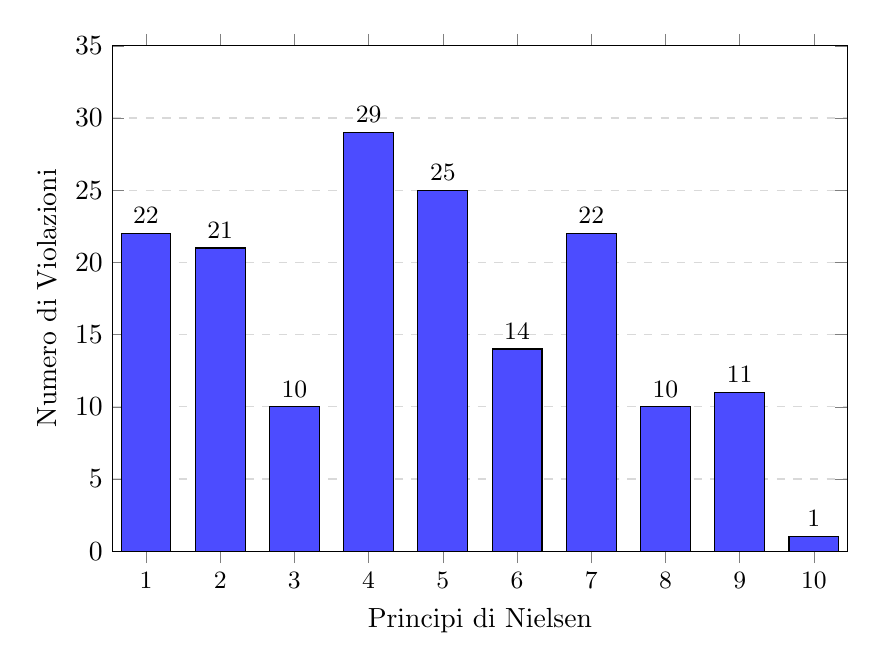
\begin{tikzpicture}
    \begin{axis}[
        ybar,
        bar width=18pt,
        width=0.9\textwidth,
        height=8cm,
        symbolic x coords={P1, P2, P3, P4, P5, P6, P7, P8, P9, P10},
        xtick=data,
        xticklabels={1, 2, 3, 4, 5, 6, 7, 8, 9, 10},
        x tick label style={font=\small},
        xlabel={Principi di Nielsen},
        ylabel={Numero di Violazioni},
        ymin=0,
        ymax=35,
        ymajorgrids=true,
        grid style={dashed, gray!30},
        enlarge x limits=0.05,
        nodes near coords,
        every node near coord/.style={font=\small, color=black},
      ]
      \addplot+[ybar, fill=blue!70, draw=black] coordinates {
        (P1,22)
        (P2,21)
        (P3,10)
        (P4,29)
        (P5,25)
        (P6,14)
        (P7,22)
        (P8,10)
        (P9,11)
        (P10,1)
      };
    \end{axis}
  \end{tikzpicture}
  \caption{Distribuzione dei principi di Nielsen riscontrati.}
  \label{fig:violazioni-nielsen}
\end{figure}

Dall'analisi del grafico emerge uno scenario chiaro sulle problematiche di \textit{BrainBox}, con una concentrazione di violazioni su principi specifici:

\begin{itemize}
  \item \textbf{Assicurare consistenza (p4 - 29 violazioni):} È la criticità principale.
    Il sistema presenta numerose incoerenze: termini diversi per indicare la stessa funzione
    e stili grafici differenti tra le sezioni.
    Questo rende difficile per l'utente comprendere come funziona il sistema.

  \item \textbf{Riconoscimento piuttosto che uso della memoria (p5 - 25 violazioni):}
    L'interfaccia richiede all'utente di ricordare informazioni da una pagina all'altra
    invece di mostrarle quando necessario. Questo aumenta il carico cognitivo e rende
    l'utilizzo del sistema più complesso.

  \item \textbf{Visualizzare tutte e sole le informazioni necessarie (p7 - 22 violazioni):}
    L'interfaccia presenta troppi elementi che distraggono l'utente dall'obiettivo principale,
    oppure mancano gerarchie chiare per distinguere le informazioni importanti da quelle secondarie.

  \item \textbf{Far vedere lo stato del sistema (p1 - 22 violazioni):} Il sistema non fornisce feedback
    adeguato all'utente, che rimane incerto sull'esito delle operazioni (es. durante il caricamento di file audio).

  \item \textbf{Adeguare il sistema al mondo reale (p2 - 21 violazioni):} Il sistema presenta
    testi in lingua inglese non tradotti, icone poco intuitive e titoli fuorvianti che ostacolano la comprensione immediata delle funzionalità da parte degli utenti.
\end{itemize}

Per una visione d'insieme più sintetica, nel grafico sottostante è mostrata la distribuzione percentuale delle tre principali categorie in cui si suddividono i principi di Nielsen.

\begin{figure}[H]
  \centering
  \begin{tikzpicture}

    % ---- PIE CHART (percentuali corrette) ----
    \pie[
      color={blue!55!white, red!50!white, green!55!white},
      radius=2.3,
      text=,     % <-- questa riga evita il testo dentro gli spicchi
      rotate=20
    ]{
      32.1/Percezione,
      54.6/Cognizione,
      13.3/Errori
    }

    % ---- LEADER LINES + LABELS (violazioni reali) ----

    % Angoli medi con rotate=20:
    % Percezione ~57°
    % Cognizione ~213°
    % Errori ~336°

    % --- Percezione ---
    \draw[thick] (57:2.3) -- ++(57:0.6) -- +(0.6,0)
    node[right]{\textbf{Percezione} (53 violazioni)};

    % --- Cognizione ---
    \draw[thick] (213:2.3) -- ++(213:0.6) -- +(-0.6,0)
    node[left]{\textbf{Cognizione} (90 violazioni)};

    % --- Errori ---
    \draw[thick] (336:2.3) -- ++(336:0.6) -- +(0.6,0)
    node[right]{\textbf{Errori} (22 violazioni)};

  \end{tikzpicture}
  \caption{Classificazione dei problemi riscontrati per categoria di appartenenza.}
  \label{fig:categorie-principi-nielsen}
\end{figure}

Dal grafico emerge chiaramente che la maggior parte dei problemi riguarda la categoria \textbf{Cognizione}, che comprende le violazioni sui principi 4,5,6,7.
Questo indica che le difficoltà principali non sono di natura tecnica, ma cognitive: l'utente deve fare uno sforzo eccessivo per comprendere e utilizzare il sistema.

La categoria \textbf{Percezione} include i problemi che violano i principi 1,2,3. Questi problemi rendono difficile individuare le informazioni necessarie a causa di un'interfaccia disordinata o della mancanza di feedback visivi.

La categoria \textbf{Errori} è la meno frequente e comprende le violazioni sui principi 8,9,10. Nonostante il numero ridotto, questi problemi possono bloccare completamente l'utilizzo del sistema quando si verificano.



\begin{figure}[H]
  \centering
  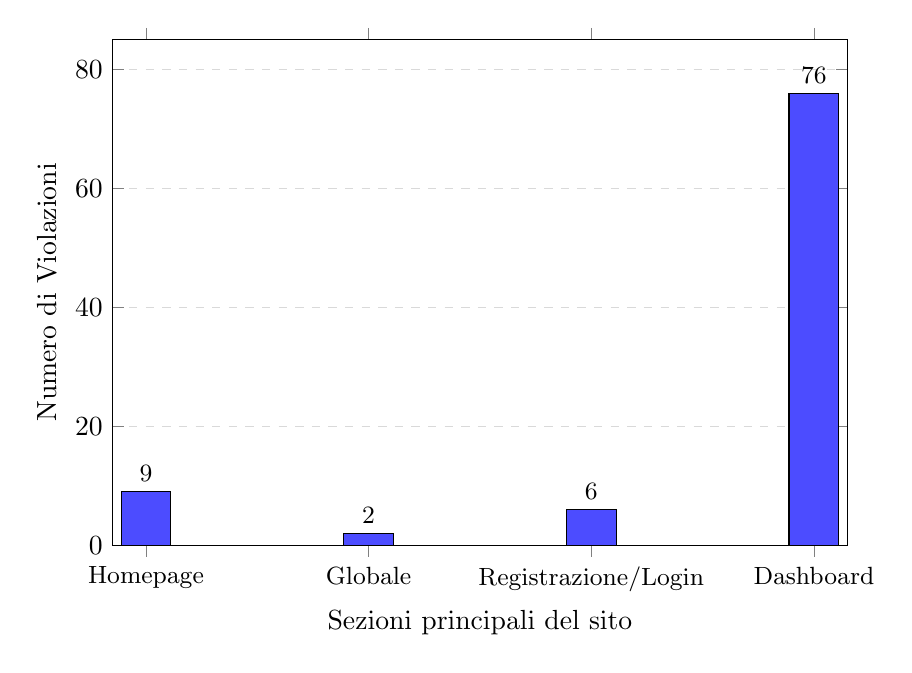
\begin{tikzpicture}
    \begin{axis}[
        ybar,
        bar width=18pt,
        width=0.9\textwidth,
        height=8cm,
        symbolic x coords={P1, P2, P3, P4},
        xtick=data,
        xticklabels={Homepage, Globale, Registrazione/Login, Dashboard},
        x tick label style={font=\small},
        xlabel={Sezioni principali del sito},
        ylabel={Numero di Violazioni},
        ymin=0,
        ymax=85,
        ymajorgrids=true,
        grid style={dashed, gray!30},
        enlarge x limits=0.05,
        nodes near coords,
        every node near coord/.style={font=\small, color=black},
      ]
      \addplot+[ybar, fill=blue!70, draw=black] coordinates {
        (P1,9)
        (P2,2)
        (P3,6)
        (P4,76)
      };
    \end{axis}
  \end{tikzpicture}
  \caption{Classificazione dei problemi riscontrati per sezione di appartenenza.}
  \label{fig:violazioni-sezioni-sito}
\end{figure}

Come si può osservare, la \textit{Dashboard} presenta il numero più elevato di violazioni, con ben 76 problematiche identificate, rappresentando così l'area più critica del sito in termini di usabilità.
La \textit{Homepage} registra 9 violazioni, posizionandosi come la seconda sezione più problematica, sebbene con un numero significativamente inferiore rispetto alla \textit{Dashboard}.
Le sezioni di \textit{Registrazione/Login} presenta 6 violazioni, mentre a livello \textit{Globale} risultano esserci solo 2 violazioni rilevate.
La marcata differenza tra il numero di violazioni nelle sezioni della \textit{Dashboard} e nelle altre sezioni suggerisce che questa area del sito, caratterizzata da una maggiore complessità funzionale e interattiva, richiede un'attenzione particolare per garantire un'esperienza fruibile e usabile da tutti gli utenti. \\

\noindent
Considerato che la \textit{Dashboard} rappresenta la sezione del sito con il maggior numero di violazioni rilevate, si è reso necessario un approfondimento più dettagliato di quest'area. Per questo motivo, è stato elaborato un ulteriore grafico che suddivide e analizza la distribuzione dei problemi di usabilità all'interno delle singole sezioni che la compongono.

\begin{figure}[H]
  \centering
  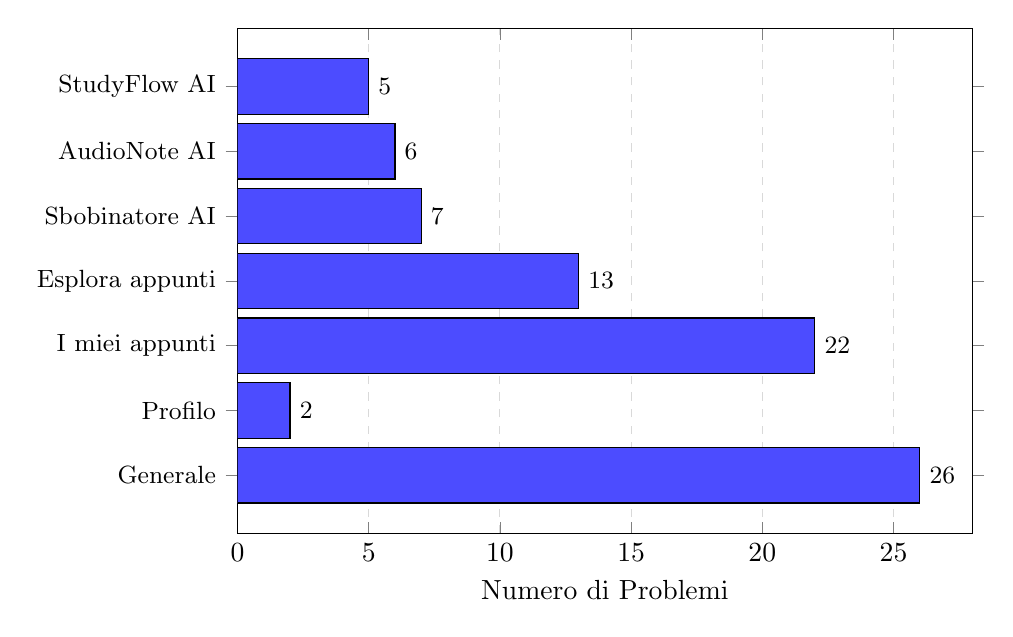
\begin{tikzpicture}
    \begin{axis}[
        xbar,
        bar width=20pt,
        width=0.9\textwidth,
        height=8cm,
        symbolic y coords={S0, S1, S2, S3, S4, S5, S6},
        ytick=data,
        yticklabels={Generale, Profilo, I miei appunti, Esplora appunti, Sbobinatore AI, AudioNote AI, StudyFlow AI},
        y tick label style={font=\small},
        xlabel={Numero di Problemi},
        xmin=0,
        xmax=28,
        xmajorgrids=true,
        grid style={dashed, gray!30},
        enlarge y limits=0.15,
        nodes near coords,
        every node near coord/.style={font=\small, color=black},
      ]
      \addplot+[xbar, fill=blue!70, draw=black] coordinates {
        (26,S0)
        (2,S1)
        (22,S2)
        (13,S3)
        (7,S4)
        (6,S5)
        (5,S6)
      };
    \end{axis}
  \end{tikzpicture}
  \label{fig:problemi-Dashboard}
  \caption{Distribuzione dei problemi di usabilità rilevati nelle diverse sezioni della Dashboard.}
\end{figure}

Come si può osservare, la sezione \textit{I miei appunti} presenta il numero più elevato di violazioni, con ben 22 problematiche identificate, rappresentando così l'area più critica dell'applicazione in termini di usabilità.
I problemi di natura generale, che interessano trasversalmente l'intera piattaforma, ammontano a 26 violazioni, costituendo una categoria significativa che richiede interventi sistemici.
La sezione \textit{Esplora appunti} registra 13 violazioni, posizionandosi come la terza area più problematica, seguita dalle funzionalità AI: \textit{Sbobinatore AI} con 7 violazioni, \textit{AudioNote AI} con 6 e \textit{StudyFlow AI} con 5.
La sezione \textit{Profilo} risulta essere la meno problematica tra le pagine specifiche, con sole 2 violazioni rilevate.
La marcata concentrazione di problematiche nella sezione \textit{I miei appunti} e nei problemi generali suggerisce che queste aree, caratterizzate da una maggiore complessità funzionale e da un impatto trasversale sull'esperienza utente, richiedono un'attenzione particolare per garantire un'esperienza fruibile e usabile da tutti gli utenti.


--------------------------------------------------------------
\begin{figure}[H]
  \centering
  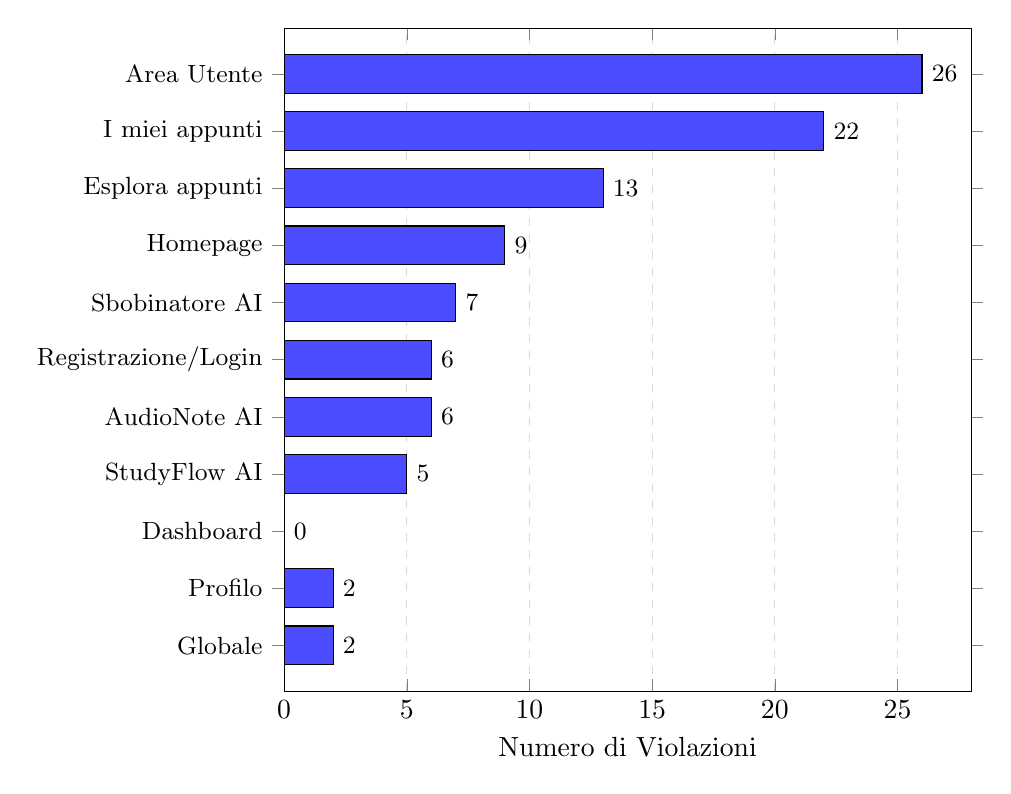
\begin{tikzpicture}
    \begin{axis}[
        xbar,
        bar width=14pt,
        width=0.85\textwidth,
        height=10cm,
        symbolic y coords={
          Globale,
          Profilo,
          Dashboard, % <-- Da aggiornare con il valore reale
          StudyFlow AI,
          AudioNote AI,
          Registrazione/Login,
          Sbobinatore AI,
          Homepage,
          Esplora appunti,
          I miei appunti,
          Area Utente
        },
        ytick=data,
        y tick label style={font=\small},
        xlabel={Numero di Violazioni},
        xmin=0,
        xmax=28,
        xmajorgrids=true,
        grid style={dashed, gray!30},
        enlarge y limits=0.08,
        nodes near coords,
        nodes near coords align={horizontal},
        every node near coord/.style={font=\small, color=black},
      ]
      % I dati sono inseriti dal più piccolo al più grande per far apparire 
      % la barra più lunga in alto nel grafico
      \addplot+[xbar, fill=blue!70, draw=black] coordinates {
        (2,Globale)
        (2,Profilo)
        (0,Dashboard) % <--- INSERISCI QUI IL NUMERO DI PROBLEMI DELLA VERA DASHBOARD
        (5,StudyFlow AI)
        (6,AudioNote AI)
        (6,Registrazione/Login)
        (7,Sbobinatore AI)
        (9,Homepage)
        (13,Esplora appunti)
        (22,I miei appunti)
        (26,Area Utente)
      };
    \end{axis}
  \end{tikzpicture}
  \caption{Distribuzione completa dei problemi di usabilità per sezione del sistema.}
  \label{fig:violazioni-complete}
\end{figure}

L'analisi della distribuzione fisica delle criticità è stata consolidata in un'unica vista complessiva (Figura \ref{fig:violazioni-complete}), permettendo di mappare l'incidenza dei problemi sull'intera architettura informativa del sistema, dall'area pubblica fino alle specifiche funzionalità dell'area personale.

Come si evince chiaramente dal grafico, le violazioni non si concentrano prevalentemente su singole pagine isolate, bensì su elementi condivisi. La categoria \textit{Trasversale (Area Utente)} risulta essere la più critica con 26 problematiche: si tratta di difetti di usabilità (es. incongruenze nei menù di navigazione o mancate indicazioni di stato) che l'utente sperimenta costantemente muovendosi tra le varie sezioni del proprio spazio di lavoro. A questi si sommano 2 problemi di natura puramente \textit{Trasversale (Intero sito)}, presenti sia nell'area pubblica che in quella privata.

Passando all'analisi delle pagine specifiche, la sezione \textit{I miei appunti} emerge in assoluto come l'area funzionale più problematica, registrando ben 22 violazioni. Essendo il cuore operativo della piattaforma, questa concentrazione di errori rappresenta un grave ostacolo alla fluidità dell'esperienza utente. A seguire si posiziona la sezione \textit{Esplora appunti} (13 violazioni), legata alle dinamiche di esplorazione e interazione con la community. 

Risulta interessante notare come l'area pubblica pre-login (\textit{Homepage} con 9 violazioni e \textit{Registrazione/Login} con 6) e le funzionalità avanzate basate sull'Intelligenza Artificiale (\textit{Sbobinatore AI}, \textit{AudioNote AI} e \textit{StudyFlow AI}) si assestino su valori medi, compresi tra 5 e 9 problematiche ciascuna. Infine, la pagina \textit{Profilo} e la \textit{Dashboard} riassuntiva [modifica questa frase in base al numero di problemi della dashboard] si confermano come gli ambienti più stabili e privi di frizioni del sistema.

Questa marcata polarizzazione suggerisce che gli interventi di riprogettazione dovranno concentrarsi prioritariamente sull'armonizzazione dei pattern visivi e navigazionali dell'intera area privata e, nello specifico, sul flusso di gestione dei propri documenti.